%================================================================
%\chapter{Inference Engines}\label{chap:infeng}
\chapter*{Bayesian Computation}\label{chap:infeng}
%================================================================


%================================================================
\section{Inference Engines}
%================================================================ 

While conceptually simple, Bayesian methods can be mathematically and numerically challenging. The main reason is that the marginal likelihood, the denominator in Bayes' theorem (see equation 1.4), usually takes the form of an intractable or computationally-expensive integral to solve. For this reason, the posterior is usually estimated numerically using algorithms from the Markov Chain Monte Carlo (MCMC) family or, more recently, variational algorithms. These methods are sometimes called inference engines, because, at least in principle, they are capable of approximating the posterior distribution for any probabilistic model. 

There are several methods to numerically compute the posterior. I have ordered them into two broad groups: Non-Markovian methods (Grid computing, Quadratic approximation, Variational methods) and Markovian methods (Metropolis-Hastings, Hamiltonian Monte Carlo, Sequential Monte Carlo). We will not discuss non-Markovian methods as the focus of this thesis is MCMC methods.

%================================================================
\subsection{Markov Chain Monte Carlo Methods}
%================================================================ 



There is a family of related methods, collectively known as MCMC methods. These stochastic methods allow us to get samples from the true posterior distribution as long as we are able to compute the likelihood and the prior point-wise. While this is the same condition that we need for the grid-approach, MCMC methods outperform the grid approximation. The is because MCMC methods are capable of taking more samples from higher-probability regions than lower ones. In fact, an MCMC method will visit each region of the parameter-space in accordance to their relative probabilities.

To understand what MCMC methods are, we are going to split the method into the two MC parts; the Monte Carlo part and the Markov Chain part.

%================================================================
\subsection{Diagnosing Markov Chains}
%\section{Diagnosing Posterior Samples}
%================================================================ 


%================================================================
\subsection{Other methods}
%\section{Diagnosing Posterior Samples}
%================================================================

NUTS

%================================================================
\section{Density Estimation}\label{sec:dens_est}
%================================================================

The probability density function (pdf) is a fundamental concept in statistics. In the following, we will discuss \textit{density estimation}, i.e., how to construct an estimate of the pdf from sample data. The likelihood-free inference methods are based on sampling parameters and estimating the posterior from the samples, and hence is density estimation a crucial topic to address. As we will see, density estimation can give representations that have qualitatively different features and lead to entirely different interpretation of the data. 

%================================================================
\subsection{Histograms}\label{sec:histograms}
%================================================================ 

The most basic density estimator is the histogram. Standard histograms simply partition $x$ into $k$ bins of width $h$ and then count the number $m_j$ observations of $x$ falling in bin $j$. In a more general mathematical sense, the histogram density estimator is defined as follows. Let $p$ be a pdf on an interval $I$, finite or infinite. Given an origin $x_0 \in I$ and bin width $h>0$, let $m_j$ be the number of $x$'s falling in the $j$th bin interval  $[x_0 + jh, x_0 + (j+1)h)$. The histogram density estimator at point $x$ is then:

\begin{equation*}
    \hat{p}_j(x) = \frac{m_j}{n h}
\end{equation*}


---

The most basic density estimator is the histogram [1]. A histogram is an approximate representation of data that divides the data into discrete bins and counts the number of points that fall in each bin. In a more general mathematical sense, a histogram is defined as follows [1]. We denote the density estimator by $\hat{f}$ and assume we are given a sample of $n$ observations $X_1, ..., X_n$ whose underlying density is to be estimated. Given an origin $x_0$ and a bin width $h$, the bins of the histogram are defined as the intervals $[x_0 + mh, x_0 + (m+1)h)$ for $m$ positive and negative integers. The histogram is then defined by

\begin{equation*}
    \hat{f}(x) = \frac{1}{nh} \times (\text{no. of } X_i \text{ in the same bin as } x)
\end{equation*}

The histogram can be generalized by allowing the bin widths to vary. Then the estimate becomes 

\begin{equation*}
    \hat{f}(x) = \frac{1}{n} \times \frac{(\text{no. of } X_i \text{ in the same bin as } x)}{\text{width of bin containing }x}
\end{equation*}

For instance, if we create some data that is drawn from a mixture density of two normal distributions, a simple  histogram, that is normalized such that the height of the bins reflects density instead of counts and have equal-width bins, will give the following representation of the data: 

\begin{figure}[H]
    \centering
    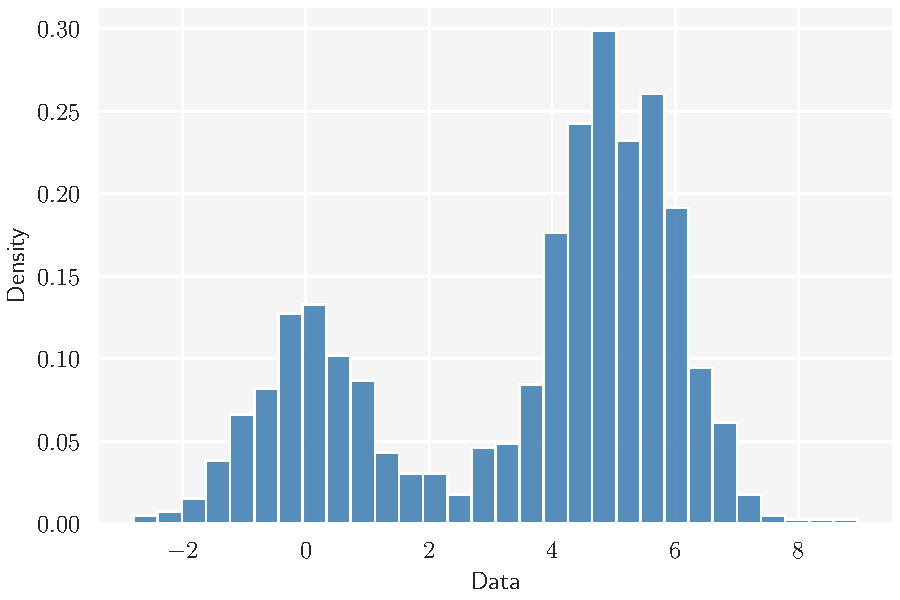
\includegraphics[scale=0.6]{bimodal_data.pdf}
    \caption{Density estimation by the histogram density estimator of 1000 observed data samples drawn from a mixed density of two normal distributions divided into 30 bins.}
    \label{fig:bimodal_data}
    \source{jakevdp book}
\end{figure}

The preceding figure illustrates why histograms are an immensely useful class of density estimates; they visualize data in an intuitive manner which is key for the presentation and exploration of data. The histogram makes clear that the data is drawn from a bimodal normal distribution.

One of the issues with using a histogram as a density estimator, however, is that the exact visual appearance depends on the choice of bin width (or number of bins) [2]. Different bin widths can give representations that have qualitatively different features and lead to entirely different interpretation of the data. Consider the following example where we draw 20 samples from the same distribution as before and use two histograms with different bin widths as density estimators:

\begin{figure}[H]
    \centering
    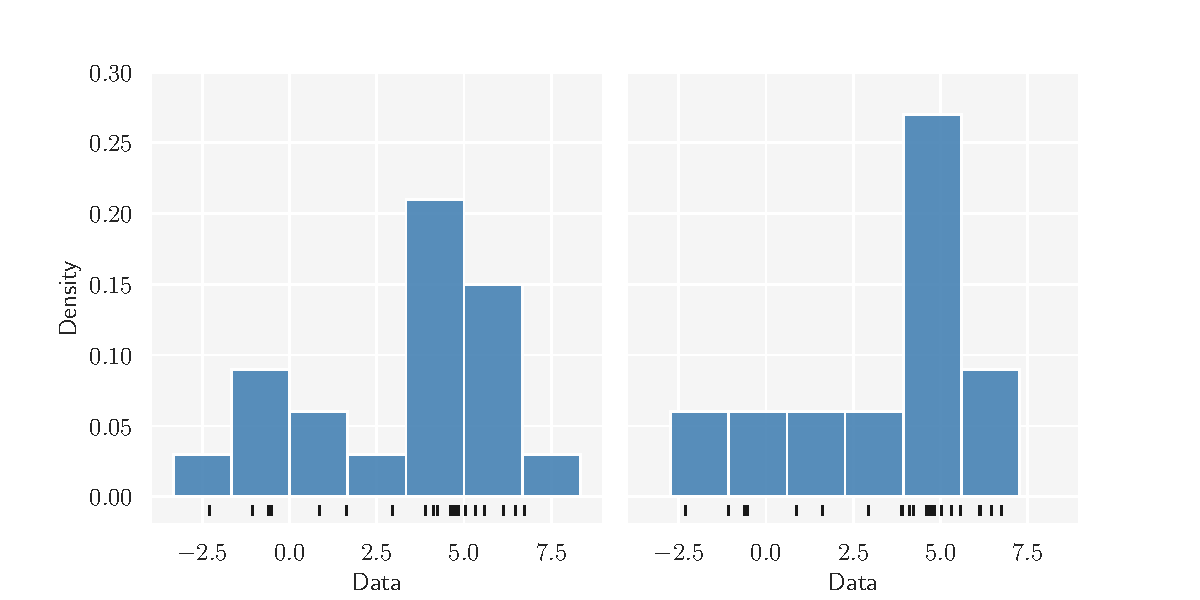
\includegraphics[scale=0.6]{bimodal_bins.pdf}
    \caption{These histograms are built from the same data, but with different bin widths. Together they illustrate one of the issues with using histograms as density estimators; the choice of bin widths can lead to vastly different representations of the data.}
    \label{fig:bimodal_bins}
    \source{jakevdp book}
\end{figure}

Without knowing that these two histograms were built from the same data, we probably would not have guessed so. The histogram on the left indicates a bimodal distribution as before, but the histogram on the right only shows a unimodal distribution with a long tail.   


%================================================================
\subsection*{Number of Bins and Width}\label{sec:binning}
%================================================================ 


There are no hard-and-fast rules concerning the bin width, and in extension the number of bins [3, p. 16]. The number of bins $k$ can be assigned directly or can be calculated from a suggested bin width $h$ as:

\begin{equation}
    k = \left \lceil \frac{\mathrm{max}\, x - \mathrm{min}\, x}{h} \right \rceil, 
\end{equation}

where $x$ is the sample data with $n$ observations. The braces indicate the ceiling function.

Smaller bin widths can make the histogram cluttered and larger bin widths may obscure nuances in the data. There are however some commonly-used rules-of-thumb, each of which has its own strengths and weaknesses. 

\subsubsection*{The Square-root Rule}

Generally, the larger the number of observations in the sample data, the more bins should be used [3, p. 16]. A reasonable rule of thumb is to take the square root of the number of observations in the sample and round to the next integer:

\begin{equation}
    k = \left \lceil \sqrt{n} \right \rceil 
\end{equation}

\textbf{Pros and Cons:} TODO

\subsubsection{Sturges' Rule}

\textbf{Rewrite, borrowed in it's entirety from Wikipedia}

Sturges' formula is derived from a binomial distribution and implicitly assumes an approximately normal distribution.

\begin{equation}
    k = \left \lceil \log_2 n \right \rceil + 1 
\end{equation}

It implicitly bases the bin sizes on the range of the data and can perform poorly if $n < 30$, because the number of bins will be small — less than seven — and unlikely to show trends in the data well. It may also perform poorly if the data are not normally distributed.

\subsubsection{Scott's Rule}

\begin{equation}
    h = \frac{3.49 \hat{\sigma}}{\sqrt[3]{n}},
\end{equation}

where $\hat{\sigma}$ is the sample standard deviation. Scott's normal reference rule is optimal for random samples of normally distributed data, in the sense that it minimizes the integrated mean squared error of the density estimate. 

\subsubsection{Freedman-Diaconis Rule}

\begin{equation}
    h = 2 \frac{\mathrm{IQR}(x)}{\sqrt[3]{n}},
\end{equation}

which is based on the interquartile range, denoted by $\mathrm{IQR}$. It replaces $3.5\sigma$ of Scott's rule with $2\,\mathrm{IQR}$, which is less sensitive than the standard deviation to outliers in data.

\subsubsection{Knuth's Rule}

Knuth's rule is a fixed-width, Bayesian approach to determining the optimal bin width of a histogram. The optimal number of bins is the value $M$ which maximizes the function 

\begin{equation}
    F(M \mid x, I) = n \log(M) + \log \Gamma \left(\frac{M}{2} \right) - \log \Gamma \left(\frac{1}{2} \right) - \log \Gamma \left(\frac{2n + M}{2} \right) + \sum_{k=1}^{M} \log \Gamma \left(n_k \frac{1}{2} \right),
\end{equation}

where $\Gamma$ is the gamma function, $n$ is the number of data points, $n_k$ is the number of measurements in bin $k$.


\begin{figure}[H]
    \centering
    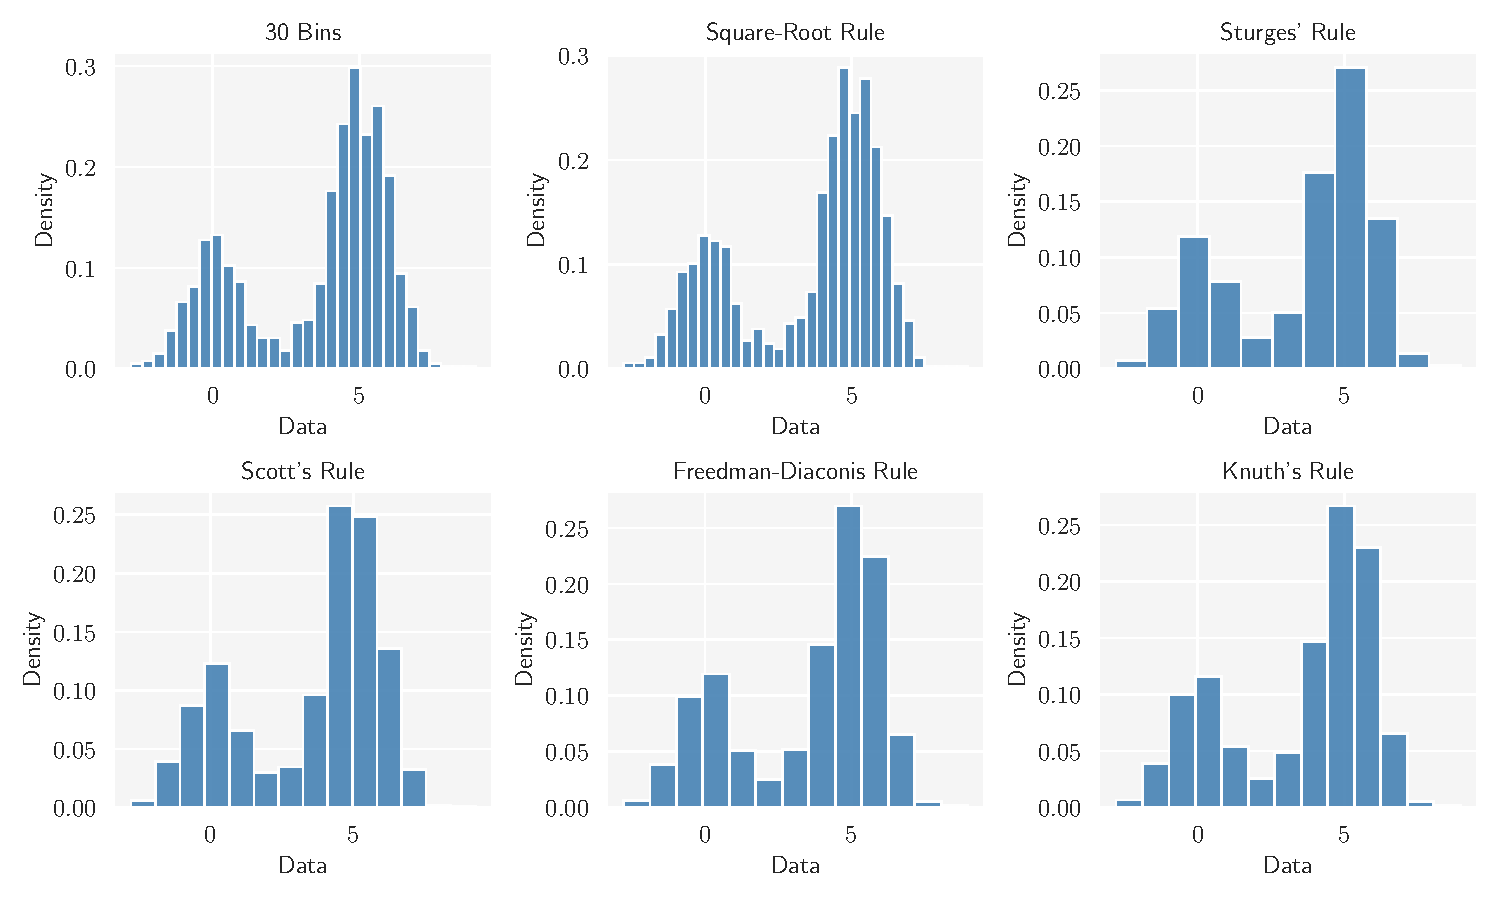
\includegraphics[scale=0.6]{histogram_rules.pdf}
    \caption{Histograms with binning as dictated by the rule specified in the subplot titles.}
    \label{fig:histogram_rules}
\end{figure}


\subsection*{References}

[1] \url{https://ned.ipac.caltech.edu/level5/March02/Silverman/paper.pdf}

[2] Python Data Science Handbook by Jake VanderPlas

[3] STK bok

[4] \url{https://clauswilke.com/dataviz/histograms-density-plots.html}

\subsubsection*{Original papers:} 

Scott, D. (1979). On optimal and data-based histograms \url{http://biomet.oxfordjournals.org/content/66/3/605}

Freedman, D. and Diaconis, P. (1981). On the histogram as a density estimator: L2 theory \url{http://www.springerlink.com/content/mp364022824748n3/}

\textbf{See also SNL thesis:} Primer on density estimation (parametric/non-parametric) and includes neural density estimators. 

\subsubsection*{Misc. sources:}

\begin{itemize}
    \item Python Data Science Handbook by Jake VanderPlas
    \item \url{https://clauswilke.com/dataviz/histograms-density-plots.html}
    \item \url{https://ned.ipac.caltech.edu/level5/March02/Silverman/paper.pdf}
    \item \url{http://users.stat.ufl.edu/~rrandles/sta6934/smhandout.pdf}
    \item \url{https://jakevdp.github.io/PythonDataScienceHandbook/04.05-histograms-and-binnings.html}
    \item \url{https://jakevdp.github.io/PythonDataScienceHandbook/05.13-kernel-density-estimation.html}
    \item \url{https://towardsdatascience.com/histograms-and-density-plots-in-python-f6bda88f5ac0}
    \item \url{https://seaborn.pydata.org/tutorial/distributions.html}
    \item \url{https://www.astroml.org/user_guide/density_estimation.html#kernel-density-estimation}
    \item \url{https://docs.astropy.org/en/stable/visualization/histogram.html#bayesian-models}
    \item \url{https://machinelearningmastery.com/probability-density-estimation/}
    \item \url{https://stackoverflow.com/questions/33458566/how-to-choose-bins-in-matplotlib-histogram/33459231}
    \item \url{https://stackoverflow.com/questions/30145957/plotting-2d-kernel-density-estimation-with-python}
\end{itemize}



\subsection*{Notes}

Histograms give a rough sense of the density of the underlying distribution of the data, and often for density estimation: estimating the probability density function of the underlying variable. The total area of a histogram used for probability density is always normalized to 1. If the length of the intervals on the x-axis are all 1, then a histogram is identical to a relative frequency plot.

A histogram can be thought of as a simplistic kernel density estimation, which uses a kernel to smooth frequencies over the bins. This yields a smoother probability density function, which will in general more accurately reflect distribution of the underlying variable. The density estimate could be plotted as an alternative to the histogram, and is usually drawn as a curve rather than a set of boxes. Histograms are nevertheless preferred in applications, when their statistical properties need to be modeled. The correlated variation of a kernel density estimate is very difficult to describe mathematically, while it is simple for a histogram where each bin varies independently. 

Though rules-of-thumb like Scott’s rule and the Freedman-Diaconis rule are fast and convenient, their strong assumptions about the data make them suboptimal for more complicated distributions. Other methods of bin selection use fitness functions computed on the actual data to choose an optimal binning. Astropy implements two of these examples: Knuth’s rule (implemented in knuth\_bin\_width()) and Bayesian Blocks (implemented in bayesian\_blocks()).

\url{https://docs.astropy.org/en/stable/visualization/histogram.html?fbclid=IwAR1qgq-CS2YLA3ui_03P9oRDcKiHXf7XE5lLYuglSjtLEXjtDSp7QBAKYag#bayesian-models}

\url{https://www.astroml.org/user_guide/density_estimation.html?fbclid=IwAR24wrXL_hTLJ8iLkzfMczUc7nUAc5elXgxpimT-A341NVaYuNKHJalXKsA#kernel-density-estimation}

\url{https://seaborn.pydata.org/tutorial/distributions.html?fbclid=IwAR3VjoNoDOcWeaERXvICVx_NL9DJ-tqhd1gBW6emPrrffgD1-0sZwtzn91I}


A rug plot is a plot of data for a single quantitative variable, displayed as marks along an axis. It is used to visualise the distribution of the data. As such it is analogous to a histogram with zero-width bins, or a one-dimensional scatter plot.

Rug plots are often used in combination with two-dimensional scatter plots by placing a rug plot of the x values of the data along the x-axis, and similarly for the y values. This is the origin of the term "rug plot", as these rug plots with perpendicular markers look like tassels along the edges of the rectangular "rug" of the scatter plot.

%================================================================
\subsection{Kernel Density Estimation}\label{sec:kde}
%================================================================

Histograms have been a popular visualization option since at least the 18th century, in part because they are easily generated by hand. More recently, as extensive computing power has become available in everyday devices such as laptops and cell phones, we see them increasingly being replaced by density plots. In a density plot, we attempt to visualize the underlying probability distribution of the data by drawing an appropriate continuous curve (Figure 7.3). This curve needs to be estimated from the data, and the most commonly used method for this estimation procedure is called kernel density estimation. In kernel density estimation, we draw a continuous curve (the kernel) with a small width (controlled by a parameter called bandwidth) at the location of each data point, and then we add up all these curves to obtain the final density estimate

Analogous to the binwidth of a histogram, a density plot has a parameter called the bandwidth that changes the individual kernels and significantly affects the final result of the plot. The plotting library will choose a reasonable value of the bandwidth for us (by default using the ‘scott’ estimate)

With many data points the rug plot can become overcrowded, but for some datasets, it can be helpful to view every data point. The rug plot also lets us see how the density plot “creates” data where none exists because it makes a kernel distribution at each data point. These distributions can leak over the range of the original data and give the impression that Alaska Airlines has delays that are both shorter and longer than actually recorded. We need to be careful about this artifact of density plots and point it out to viewers!


\url{https://github.com/COINtoolbox/CosmoABC/blob/master/cosmoabc/weighted_gaussian_kde.py} see set bandwidth function 


%=============================================================== 
\section{Likelihood-Based vs. Simulation-Based}
%=============================================================== 

Suppose a data-generating process is controlled by parameters $\theta$. When the process is run forward it stochastically generates a datapoint $y$ whose distribution depends on $\theta$. For every setting of $\theta$, assume that the process defines a conditional density function $\lhood$. Given an observed datapoint $y_0$ known to be generated by the process, the problem of interest is inferring plausible parameter settings that could have generated $y_0$. In particular, computing the posterior density $\pi \qty(\theta \mid y=y_0)$ obtained by Bayes theorem (\autoref{eq:bayes_theorem}) is of interest. The choice of inference algorithm primarily depends on how the data-generating process is modelled.
%\cite[p. 54]{papamakarios2019neural}. 

A purely statistical model, also known as a \textit{density model} or \textit{explicit model}, describes the conditional density function $\lhood$ of the process given values for $y$ and $\theta$. With a density model, the posterior density $\pi \qty(\theta \mid y=y_0)$ is, in general, easily evaluated using Bayes theorem. Even though the normalizing constant (or evidence) $p\qty(y_0)$ is typically intractable, samples from the posterior can be generated using a number of popular algorithms such as importance sampling and Markov chain Monte Carlo, or the posterior can be approximated with a more convenient distribution using e.g. variational inference. Such methods are referred to as \textit{likelihood-based inference methods}, as they explicitly evaluate the likelihood $\lhood$.
%\cite[p. 55]{papamakarios2019neural} \cite[p. 4]{abc_handbook}.

On the contrary, a \textit{simulator model}, also known as an \textit{implicit model}, describes how the process generates data. Many mechanical models are implicitly defined through simulator models, that is, as a set of dynamical equations and possibly a description of stochastic processes. For any parameter setting $\theta$, a simulator model can be run forward to generate independent samples from $\lhood$. Unlike for explicit density models, likelihoods are generally intractable or computationally infeasible for complex data-generating processes such as simulation-based models. The absence or complexity of the associated likelihood typically arise from it involving computationally expensive or intractable integrals, or that the simulator's internal states are unavailable. In order to perform inference in a simulator model, methods using simulations from the model rather than likelihood evaluations are needed. Such methods are referred to as \textit{likelihood-free inference methods}.
%\cite{SNL18} \cite{SNPE17} \cite[p. 55]{papamakarios2019neural}.

In general, likelihood-free methods are less efficient than likelihood-based methods as the former can require lots of simulations to produce accurate results. One of the principal topics of research in likelihood-free inference is how to obtain state-of-the-art results with fewer simulations. 
%\cite{comparison_snl_snpe}. 

\section{ABC}

Approximate Bayesian Computation (ABC) constitutes a class of computational methods rooted in Bayesian statistics that can be used to evaluate posterior distributions of model parameters without having to explicitly calculate likelihoods. ABC methods approximate the likelihood function by assessing how likely it is the model could have produced the observed data, based on comparing synthetic data generated by the simulator to the observed data. The simulations that do not reproduce the observed data within a specified tolerance are discarded \cite{ABCprimer}.
%\cite[p. ix]{abc_handbook}.

ABC methods have been successfully applied to a wide range of real-world problems, and have also paved the way for a range of other likelihood-free approaches. However, even though ABC methods are mathematically well-founded, they inevitably make assumptions and approximations whose impact needs to be carefully assessed \cite{ABCprimer}. In the following, three types of ABC methods will be discussed: the vanilla \textit{rejection ABC}, and the more sophisticated variant \textit{Markov chain Monte Carlo (MCMC) ABC}.

The choice of summary statistics is crucial for the performance of ABC methods, hence, the topic has been the subject of much research. See Blum et al. (2013) for a comprehensive review of methods for dimension reduction or statistics selection. SL and ABC methods share some requirements regarding the choice of summary statistics. More specifically, in parameter, estimation problems, the summary statistics should contain as much information as possible about the parameters, so that $\pi \qty(\theta \mid y_\mathrm{obs})$ will be approximately proportional to $\pi \qty(\theta \mid y_\mathrm{obs})$. \cite{ABC_ch20} 

%================================================================
\subsection{Rejection ABC}\label{sec:rejection_abc}
%================================================================

Given observed data $y_0$ and synthetic data $y$ generated by a simulator, let $\rho (\cdot, \cdot)$ be a distance metric (e.g., the Euclidean norm) defined in data space $\R^D$ and $\epsilon \geq 0$ be a tolerance. For small $\epsilon$, the ABC approximation to the posterior is 

\begin{equation}
    \pi \qty(\theta \mid y=y_0) \simeq \pi \qty(\theta \mid \rho \qty(y, y_0) \leq \epsilon)
\end{equation}


Rejection ABC is a rejection-sampling method for obtaining independent samples from the approximate posterior $ \pi \qty(\theta \mid \rho \qty(y, y_0) \leq \epsilon)$. It works by first sampling a set of parameters from the prior $\prior$, then simulating data under the model specified by the sampled parameters, and only accepting and retaining the sample if the distance between $y$ and $y_0$ is no more than $\epsilon$. The tolerance parameter $\epsilon$ controls the trade-off between estimation accuracy and computational efficiency. With sufficiently small $\epsilon$, and a sensible distance metric, the accepted samples follow the exact posterior more closely, though the algorithm accepts less often. On the other hand, the algorithm accepts more often with a large $\epsilon$, but the accepted samples will yield a replica of the prior.
%\cite[p. 58]{papamakarios2019neural} \cite{abc_handbook}. 

An issue with ABC in general is that the required number of simulations increases dramatically as $\epsilon$ becomes small. Moreover, likelihood-free inference also becomes challenging when the dimensionality of the data is large. A common approach to lessen this problem is to use lower-dimensional summary statistics, $S(y)$ and $S(y_0)$, that capture important features such as the mean and standard deviation, in place of raw data. %\cite{SNL18}. 

A further motivation for this approach is that real-world experiments often are interested in capturing summary statistics of the experimental data. A summary statistic that contains the same amount of information about model parameters as the whole dataset, is referred to as being a \textit{sufficient statistic} \cite{ABCprimer}. The acceptance criterion in the rejection ABC algorithm then becomes:

\begin{equation}
    \rho \qty(S(y), S(y_0))
\end{equation}

In \autoref{fig:abc_pipeline}, a conceptual overview of the rejection ABC algorithm is shown. 

\begin{figure}[H]
    \centering 
    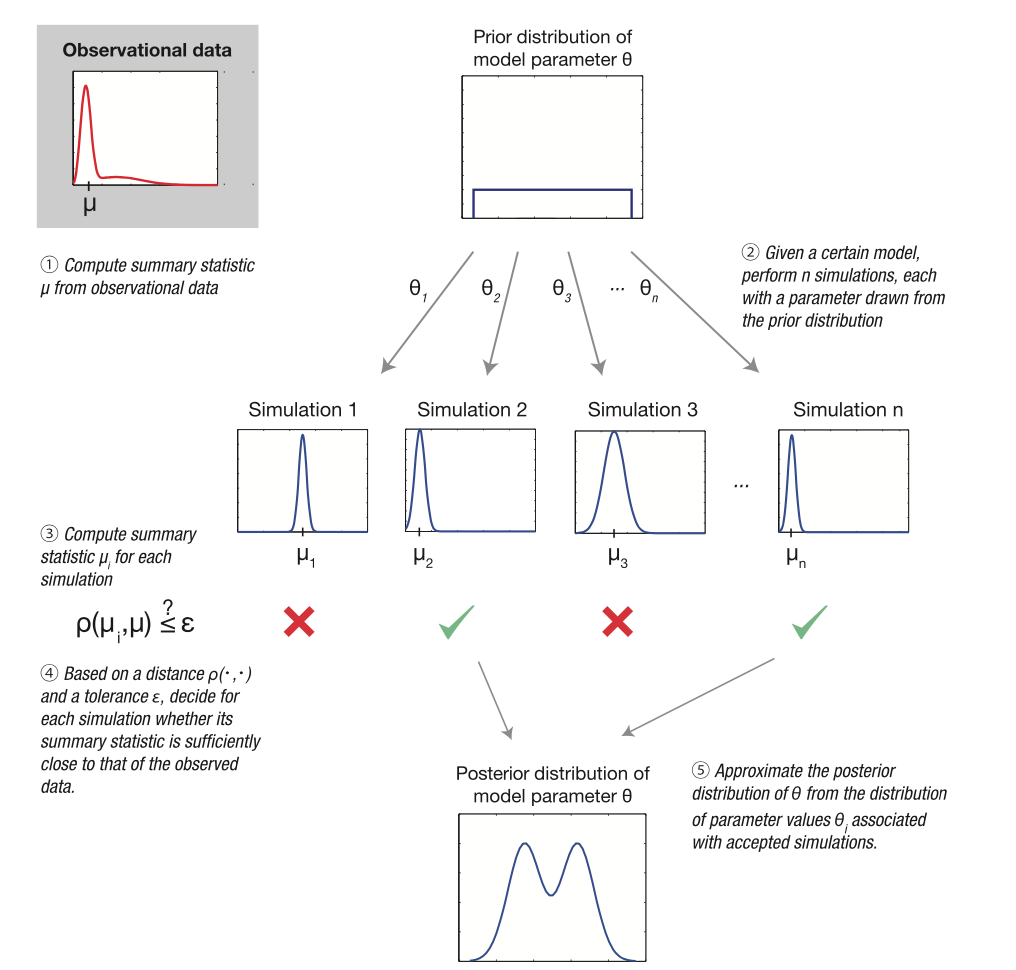
\includegraphics[scale=0.7]{./3_Images/abc_pipeline.png}
    \caption{Parameter estimation by Approximate Bayesian Computation: a conceptual overview.}
    \source{Figure 1 in \cite{ABCprimer}}
    \label{fig:abc_pipeline}
\end{figure}


\begin{algorithm}[H]
\caption{Rejection ABC}
\label{alg:mcmcabc}
\SetAlgoLined
\DontPrintSemicolon
 % Algorithm 
 \textbf{Inputs\,:}\;
 \vspace{-5mm}
 \begin{itemize}
     \item A target posterior density $\posterior \propto \lhood \prior$ consisting of a prior $\prior$ and likelihood $\lhood$. 
     \item A symmetric Markov proposal density $q \qty(\theta^* \mid \theta)$.
     \item An integer $N>0$.
 \end{itemize}
 
 \vspace{5mm}
 \textbf{Initialize\,:}\;
 Sample $\theta_0 \sim \prior$.\;

 \vspace{5mm}
 \textbf{Sampling\,:}\;
 \For{$t=1, ..., N$}{ 
 Generate proposal $\theta^* \sim q \qty(\theta^* \mid \theta_{t-1})$. \; 
 Calculate acceptance criterion $\alpha = \min \qty(1, \dfrac{p \qty(y \mid \theta^*) \pi \qty(\theta^*)}{p \qty(y \mid \theta_{t-1}) \pi \qty(\theta_{t-1})})$. \;
 Sample $u \sim \mathrm{U}(0,1)$. \; 
 \vspace{2mm}
 \eIf{$u \leq \alpha$}{
   $\theta_t = \theta^*$\;
   }{
   $\theta_t = \theta_{t-1}$\;
  }
 }
\end{algorithm}


%================================================================
\subsection{Markov Chain Monte Carlo ABC}\label{sec:mcmc_abc}
%================================================================

In the rejection ABC algorithm, parameters are sample from the prior $\prior$, and only parameters that are likely under the approximate posterior $\pi \qty(\theta \mid \rho \qty(y, y_0 ) \leq \epsilon )$ are accepted. The acceptance rate will be low if the approximate posterior is significantly narrower than the prior, as is often the case. %\cite[p. 59]{papamakarios2019neural}.

Markov-chain Monte Carlo (MCMC) ABC is an alternative approach that can lead to fewer rejections. Instead of proposing parameters from the prior, this method use the Metropolis-Hastings algorithm to propose new parameters $\theta'$ based on previously accepted parameters $\theta$ from the proposal density $q \qty(\theta' \mid \theta)$. By calculating the \textit{acceptance ratio}

\begin{equation}
    \alpha = \frac{p \qty(\rho \qty(y, y_0 ) \leq \epsilon \mid \theta') \pi\qty(\theta') q \qty(\theta \mid \theta')  }{p \qty(\rho \qty(y, y_0) \leq \epsilon \mid \theta) \pi\qty(\theta) q \qty(\theta' \mid \theta) },
\end{equation}

the algorithm outputs the proposed parameters $\theta'$ with probability $\min \qty(1, \alpha)$, otherwise it outputs the previous parameters $\theta$. 
%\cite[p. 59]{papamakarios2019neural}.

The approximate likelihood $p \qty(\rho \qty(y, y_0 ) \leq \epsilon \mid \theta)$ cannot be directly evaluated in the likelihood-free situation, but it can be estimated as the fraction of the simulated data $y$ whose distance from the observed data $y_0$ is no more than $\epsilon$:

\begin{equation}
    p \qty(\rho \qty(y, y_0) \leq \epsilon \mid \theta) \approx \frac{1}{N} \sum_n I \qty(\rho \qty(y_n, y_0) \leq \epsilon),
\end{equation}

where $y_n \sim p \qty(y \mid \theta)$ and $I(\cdot)$ is an indicator function. %\cite[p. 59]{papamakarios2019neural}.

Similarly to rejection ABC, the acceptance probability of MCMC ABC decreases as $\epsilon$ becomes small. Moreover, the performance of MCMC ABC strongly depends on the selection of proposal and prior density.

\begin{algorithm}[H]
\caption{Markov chain Monte Carlo ABC}
\label{alg:mcmcabc}
\SetAlgoLined
\DontPrintSemicolon
 % Algorithm 
 \textbf{Inputs\,:}\;
 \vspace{-5mm}
 \begin{itemize}
     \item A target posterior density $\posterior \propto \lhood \prior$ consisting of a prior $\prior$ and likelihood $\lhood$. 
     \item A symmetric Markov proposal density $q \qty(\theta^* \mid \theta)$.
     \item An integer $N>0$.
 \end{itemize}
 
 \vspace{5mm}
 \textbf{Initialize\,:}\;
 Sample $\theta_0 \sim \prior$.\;

 \vspace{5mm}
 \textbf{Sampling\,:}\;
 \For{$t=1, ..., N$}{ 
 Generate proposal $\theta^* \sim q \qty(\theta^* \mid \theta_{t-1})$. \; 
 Calculate acceptance criterion $\alpha = \min \qty(1, \dfrac{p \qty(y \mid \theta^*) \pi \qty(\theta^*)}{p \qty(y \mid \theta_{t-1}) \pi \qty(\theta_{t-1})})$. \;
 Sample $u \sim \mathrm{U}(0,1)$. \; 
 \vspace{2mm}
 \eIf{$u \leq \alpha$}{
   $\theta_t = \theta^*$\;
   }{
   $\theta_t = \theta_{t-1}$\;
  }
 }
\end{algorithm}

%================================================================
\subsection{Sequential Monte Carlo ABC}\label{sec:smc_abc}
%================================================================

TODO

%===============================================================
\subsection{Sequential Neural Posterior Estimation}
%\subsection{Neural Density Estimation}
%===============================================================

Sequential Neural Posterior Estimation (SNPE) is a novel algorithm for simulation-based inference. Dissecting all of the intricacies of SNPE is beyond the scope of this thesis. We will in this section provide an overview of the algorithm. For all details we refer the reader to the original articles \cite{SNL_first}, \cite{SNPE_first} and \cite{SNPE_apt}.

Sequential Neural Posterior Estimation (SNPE)\footnote{Source code available at \url{https://github.com/mackelab/delfi}} is a novel method for parameter inference. The method uses ABC to learn a neural network which maps features of observed data to the posterior distribution over parameters. The strategy was originally proposed by Papamakarios and Murray in \cite{papamakarios2016fast} and further developed by Lueckmann et al. in \cite{SNPE17} and \cite{SNPE19}. In the literature, the variant of Papamakarios and Murray is often referred to as SNPE-A and the variant of Lueckmann et al. as SNPE-B. In this essay, SNPE refer to the particular method by Lueckmann et al.

A \textit{conditional neural density estimator} is a parametric density model $q_{\bm{\phi}}$ (such as a neural network), where $\bm{\phi}$ are distribution parameters. With a pair of datapoints $(\bm{u}, \bm{v})$ as input, the model outputs a conditional probability density $q_{\bm{\phi}}(\bm{u}\mid \bm{v})$. Given a set of training data $\qty{\bm{u}_n, \bm{v}_n}_{1\colon N}$ that are independent and identically distributed according to a joint probability density $p(\bm{u}, \bm{v})$, $q_{\bm{\phi}}$ is trained by minimizing the loss $\mathcal{L} = - \sum_n \log q_{\bm{\phi}}(\bm{u}_n, \bm{v}_n)$ with respect to $\bm{\phi}$. With enough training data, and with a sufficiently flexible model, $q_{\bm{\phi}}(\bm{u}\mid \bm{v})$ will learn to approximate the conditional $p(\bm{u}\mid \bm{v})$ \cite{SNL18}. 

A neural density estimator $q_{\bm{\phi}}(\bm{\theta} \mid \bm{x})$ can be used to approximate the posterior $p \qty(\bm{\theta}\mid \bm{x}_0)$ as follows. First, a set of samples $\qty{\bm{\theta}_n , \bm{x}_n}_{1\colon N}$ is obtained from the joint distribution $p (\bm{\theta}, \bm{x})$, by $\bm{\theta}_n \sim \prior$ and $\bm{x}_n \sim p \qty(\bm{x} \mid \bm{\theta}_n)$ for $n=1, ..., N$. Then, $q_{\bm{\phi}}$ is trained using $\qty{\bm{\theta}_n , \bm{x}_n}_{1\colon N}$ as training data in order to a global approximation of $\posterior$. Finally, $p \qty(\bm{\theta} \mid \bm{x}_0)$ can be simply estimated by $q_{\bm{\phi}} \qty(\bm{\theta} \mid \bm{x}_0)$. In order to obtain an accurate posterior fit, this approach may require a large number of simulations to sample enough training data in the vicinity of $\bm{x}_0$ \cite{SNL18}. 

SNPE is a strategy for reducing the number of simulations needed by conditional neural estimation. Since simulations from parameters with low posterior density $p \qty(\bm{\theta} \mid \bm{x}_0)$ may not be useful in training $q_{\bm{\phi}}$, the key idea of SNPE is to generate parameter samples $\bm{\theta}_n$ from a proposal $\tilde{p}(\bm{\theta})$, that generates data $\bm{x}_n$ more likely to be in the vicinity of $\bm{x}_0$,  instead of the prior $\prior$ \cite{SNL18}. However, minimizing $\mathcal{L}$ on samples drawn from a proposal $\tilde{p}(\bm{\theta})$ no longer yields the target posterior but rather the \textit{proposal posterior}
\begin{equation}
    \tilde{p}(\bm{\theta} \mid \bm{x}) = p (\bm{\theta} \mid \bm{x}) \frac{\tilde{p}(\bm{\theta}) p(\bm{x}) }{\prior \tilde{p}(\bm{x}) },
\end{equation}
where $\tilde{p}(\bm{x}) = \int \tilde{p} (\bm{\theta}) \lhood d\bm{\theta}$ and it is assumed that $\tilde{p} (\bm{\theta})=0$ where $\prior = 0$ \cite{apt}. Hence, to account for sampling from a proposal $\tilde{p}(\bm{\theta})$, an adjustment of either the learned posterior or the proposed samples must be made. 

Lueckmann et al. deal with this problem by adjusting the parameter samples $\bm{\theta}_n$ by assigning them weights $w_n = p \qty(\bm{\theta}_n)/ \tilde{p} \qty(\bm{\theta}_n)$. During training SNPE minimizes an importance weighted loss $- \sum_n w_n \log q_{\bm{\phi}}(\bm{\theta}_n \mid \bm{x}_n)$, which allows for direct recovery of $p \qty(\bm{\theta} \mid \bm{x})$ from $q_{\bm{\phi}}$ with no correction and no restrictions on $p(\bm{\theta})$, $\tilde{p}(\bm{\theta})$ or $q_{\bm{\phi}}$ \cite{apt}. However, the weights can have a high variance, which can lead to slow or inaccurate inference \cite{SNL18}.
  
In \autoref{fig:snpe}, a conceptual overview of the SNPE method is shown.

\begin{figure}[H]
\begin{center}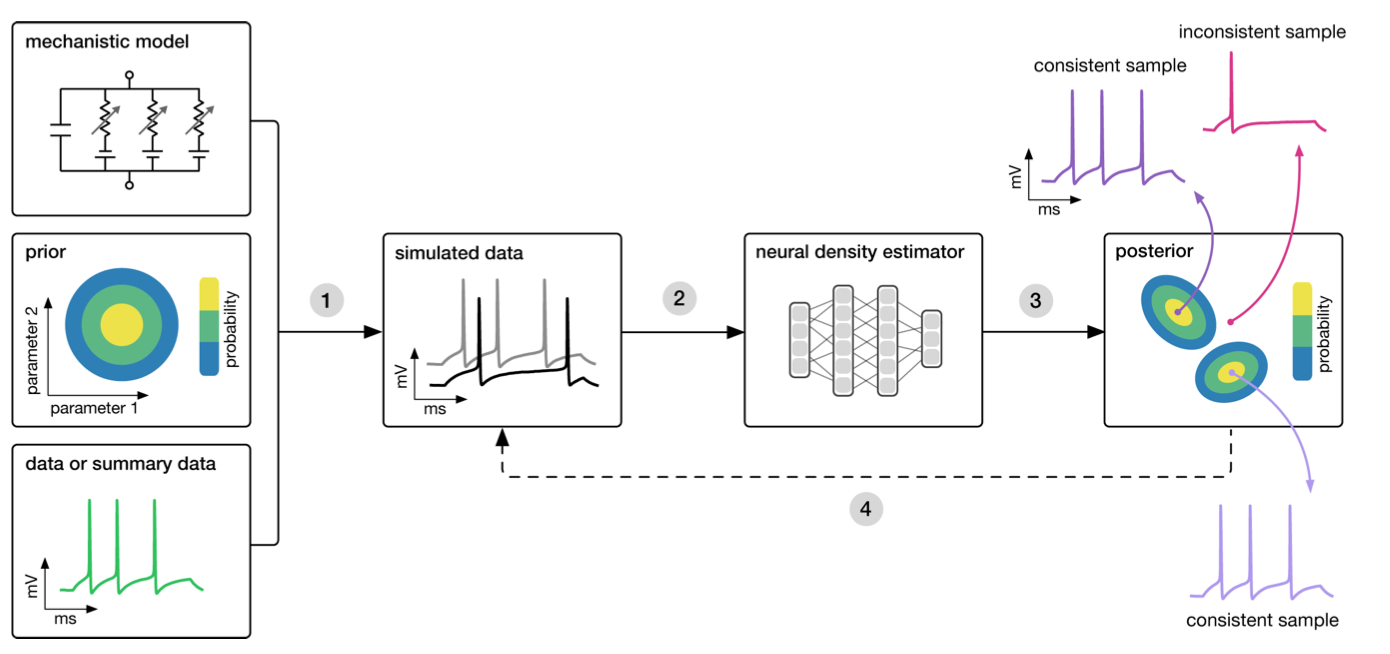
\includegraphics[scale=0.65]{snpe}
\end{center}
\caption{Parameter estimation by Sequential Neural Posterior Estimation (SNPE): a conceptual overview. Retrieved from \cite[Figure 1]{SNPE19}.}
\label{fig:snpe}
\end{figure}





%================================================================
\subsection{Population Monte Carlo ABC}\label{sec:pmc_abc}
%================================================================

TODO

\section{Notes}

\begin{itemize}
    \item See LFI for cognitive science book, Ch. 2.1
\end{itemize}

\textbf{Snippets:}

Although the steps listed above may give the impression that all likelihood- free algorithms are simple, this is unfortunately not the case. Many sophisticated techniques have been created in the hopes of increasing the efficiency of an algorithm on a given problem, and as one might expect, the efficiency of the algorithms below do vary by the type of problem to which they are applied. Because the algorithms we present later in this chapter are sometimes complex, we first introduce a few concepts at a high level by describing the different choices one can make at Steps 1, 2, or 3. 

The ABC methodology, where ABC stands for approxi- mate Bayesian computation, was mentioned as early as 1984 through a pedagogical and philosophical argument in Rubin (1984). It offers an almost automated resolution of the dif- ficulty with models which are intractable but can be simu- lated from. It was first proposed in population genetics by Tavaré et al. (1997), who introduced Approximate Bayesian Computation methods as a rejection technique bypassing the computation of the likelihood function via a simulation from the corresponding distribution. The exact version of the method can only be implemented in a small range of cases. Pritchard et al. (1999) produce a generalisation based on an approximation of the target. We study here the foundations as well as the implementation of the ABC method, with il- lustrations from time series. 

\textbf{Books/papers:} 

\begin{itemize}
    \item marin2012\_article\_abc, bra abc analyser 
\end{itemize}

LFI chapter, 2019 book statistics and data science, side 98, ligning (2): 

Unfortunately, we cannot evaluate (2) explicitly. However it is possible to drawn an IID random sample $T_N = \{ \Theta_j \}_{j=1}^N$ $(N \in \mathbb{N})$ from the quasi-posterior distribution that is characterized by (2), using the so-called rejection algorithm. 

\textbf{Links:}

\url{https://www.ncbi.nlm.nih.gov/pmc/articles/PMC4297650/}

Clearly, deciding how to characterize the data is an important choice in the likelihood-free context. Namely, it is impossible to know whether or not a set of statistics is sufficient for the unknown parameters if the likelihood is intractable.

\url{https://github.com/bmorris3/abc_interact/blob/master/abc_interact.ipynb}

\url{https://github.com/elfi-dev/elfi/blob/dev/elfi/methods/parameter_inference.py}

\textbf{MCMC} 

\url{https://github.com/davidtgonzales/ABC/blob/master/Lotka-Volterra%20ABC.ipynb}

\textbf{SMC} 

\url{https://docs.pymc.io/notebooks/SMC-ABC_Lotka-Volterra_example.html}

\url{https://github.com/pymc-devs/pymc3/tree/master/pymc3/smc}

\url{https://github.com/ICB-DCM/pyABC/blob/main/pyabc/inference/smc.py}

\url{https://github.com/vuolleko/abclib/blob/master/abclib.pyx}

\url{https://github.com/Neojume/pythonABC/blob/master/algorithms.py}


%================================================================
\section{The ABC of Approximate Bayesian Computation}\label{sec:abc_of_abc}
%================================================================

Content from notebook, source: ABC handbook

For discrete data $\mathcal{D}$, probability model $\mathcal{M}$ with parameters $\theta$ having prior $\pi(\theta)$, we can simulate observations from: 

\begin{equation}
    \pi (\theta \mid \mathcal{D}) \propto p(\mathcal{D} \mid \theta) \pi(\theta),
\end{equation}

via:

\begin{itemize}
    \item[A1] Generate $\theta \sim \pi(\theta)$
    \item[A2] Accept $\theta$ with probability proportional to the likelihood $p(\mathcal{D}\mid \theta)$
\end{itemize}
    
Algorithm A can be extended dramatically in its usefulness using the following, stochastically equivalent, version:

\begin{itemize}
    \item[B1] Generate $\theta \sim \pi(\theta)$
    \item[B2] Simulate an observation $\mathcal{D}'$ from model $\mathcal{M}$ with parameter $\theta$
    \item[B3] Accept $\theta$ if $\mathcal{D}' = \mathcal{D}$
\end{itemize}
    

While algorithms A and B are probabilistically identical, B is much more general in that one does not need to compute probabilities explicitly to make it work; only simulation is needed. Version B is due to Rubin (1984). 

The drawback of B is clear. It will typically be the case that for a given value of $\theta$, the chance of the outcome $\mathcal{D}'=\mathcal{D}$, namely $p(\mathcal{D} \mid \theta)$, is either vanishingly small or very time consuming to compute, resulting in an algorithm that does not work effectively. This is where ABC finally comes into play, in the form of the following scheme. We start with a discrepancy metric $\rho$ to compare datasets and a tolerance $\epsilon \geq 0$, and then: 

\begin{itemize}
    \item[C1] Generate $\theta \sim \pi(\theta)$
    \item[C2] Simulate an observation $\mathcal{D}'$ from model $\mathcal{M}$ with parameter $\theta$
    \item[C3] Compute $\rho \equiv \rho (\mathcal{D}', \mathcal{D})$, and accept $\theta$ as an appropriate draw from $\pi (\theta \mid \mathcal{D})$ if $\rho \leq \epsilon$
\end{itemize}
    
The parameter $\epsilon$ measures the tension between computability and accuracy. If $\rho$ is a metric, then 

\begin{equation*}
    \rho = 0 \quad \implies \quad \mathcal{D}'=\mathcal{D},
\end{equation*}

so that such an accepted $\theta$ is indeed an observation from the true posterior. 

Pritchard et al. (1999) were the first to describe a version of this scheme, in which the datasets in C3 were compared through a choice of summary statistics. Thus, $\rho$ compares how well a set of simulated summary statistics matches the observed summary statistics. If the statistics are sufficient for $\theta$, then when $\epsilon=0$, the accepted values of $\theta$ are still from the true posterior based on the full data. 

\textbf{This begs the question of how one might identify 'approximately sufficient' statistics, a topic covered in CHAPTER X.}

\subsection{Goodness of Fit}

\begin{itemize}
    \item Assessing performance 
    \item Expected quadratic loss
    \item \url{https://en.wikipedia.org/wiki/Loss_function}
    \item Expected loss
    \item In some contexts, the value of the loss function itself is a random quantity because it depends on the outcome of a random variable X.
    \item Both frequentist and Bayesian statistical theory involve making a decision based on the expected value of the loss function; however, this quantity is defined differently under the two paradigms.
\end{itemize}

\subsection{TODOs}

\begin{itemize}
    \item Sufficient vs insufficient statistics 
    \item $p(\theta \mid \rho (\hat{D}, D) \leq \epsilon)$ and $p(\theta |D)$ as a function of $\epsilon$. 
    \item The accuracy of the posterior (defined as the expected quadratic loss) delivered by ABC as a function of $\epsilon$
    \item Accuracy as a function of the number of data points in observed data
    \item KL divergence
    \item Accuracy vs number of posterior samples
\end{itemize}


\section{ABC}

The choice of summary statistics is crucial for the performance of ABC methods, hence, the topic has been the subject of much research. See Blum et al. (2013) for a comprehensive review of methods for dimension reduction or statistics selection. SL and ABC methods share some requirements regarding the choice of summary statistics. More specifically, in parameter, estimation problems, the summary statistics should contain as much information as possible about the parameters, so that $\pi \qty(\theta \mid y_\mathrm{obs})$ will be approximately proportional to $\pi \qty(\theta \mid y_\mathrm{obs})$. \cite{ABC_ch20} 


Clearly, deciding how to characterize the data is an important choice in the likelihood-free context. Namely, it is impossible to know whether or not a set of statistics is sufficient for the unknown parameters if the likelihood is intractable.

However, sufficient statistics are hard to come by, but if powerful low-dimensional summary statistics are established, ABC can still offer a reasonable performance. 

Given observed data $y_0$ and synthetic data $y$ generated by a simulator, let $\rho (\cdot, \cdot)$ be a distance metric (e.g., the Euclidean norm) defined in data space $\R^D$ and $\epsilon \geq 0$ be a tolerance. For small $\epsilon$, the ABC approximation to the posterior is 

\begin{equation}
    \pi \qty(\theta \mid y=y_0) \simeq \pi \qty(\theta \mid \rho \qty(y, y_0) \leq \epsilon)
\end{equation}


Rejection ABC is a rejection-sampling method for obtaining independent samples from the approximate posterior $ \pi \qty(\theta \mid \rho \qty(y, y_0) \leq \epsilon)$. It works by first sampling a set of parameters from the prior $\prior$, then simulating data under the model specified by the sampled parameters, and only accepting and retaining the sample if the distance between $y$ and $y_0$ is no more than $\epsilon$. The tolerance parameter $\epsilon$ controls the trade-off between estimation accuracy and computational efficiency. With sufficiently small $\epsilon$, and a sensible distance metric, the accepted samples follow the exact posterior more closely, though the algorithm accepts less often. On the other hand, the algorithm accepts more often with a large $\epsilon$, but the accepted samples will yield a replica of the prior.
%\cite[p. 58]{papamakarios2019neural} \cite{abc_handbook}. 

An issue with ABC in general is that the required number of simulations increases dramatically as $\epsilon$ becomes small. Moreover, likelihood-free inference also becomes challenging when the dimensionality of the data is large. A common approach to lessen this problem is to use lower-dimensional summary statistics, $S(y)$ and $S(y_0)$, that capture important features such as the mean and standard deviation, in place of raw data. %\cite{SNL18}.

A further motivation for this approach is that real-world experiments often are interested in capturing summary statistics of the experimental data. A summary statistic that contains the same amount of information about model parameters as the whole dataset, is referred to as being a \textit{sufficient statistic} \cite{ABCprimer}. The acceptance criterion in the rejection ABC algorithm then becomes:

\begin{equation}
    \rho \qty(S(y), S(y_0))
\end{equation}


---

The parameter $\epsilon$ measures the tension between computability and accuracy. If $\rho$ is a metric, then 

\begin{equation*}
    \rho = 0 \quad \implies \quad \mathcal{D}'=\mathcal{D},
\end{equation*}

so that such an accepted $\theta$ is indeed an observation from the true posterior. 

Pritchard et al. (1999) were the first to describe a version of this scheme, in which the datasets in C3 were compared through a choice of summary statistics. Thus, $\rho$ compares how well a set of simulated summary statistics matches the observed summary statistics. If the statistics are sufficient for $\theta$, then when $\epsilon=0$, the accepted values of $\theta$ are still from the true posterior based on the full data. 

---


\section{MCMC ABC}

In the rejection ABC algorithm, parameters are sample from the prior $\prior$, and only parameters that are likely under the approximate posterior $\pi \qty(\theta \mid \rho \qty(y, y_0 ) \leq \epsilon )$ are accepted. The acceptance rate will be low if the approximate posterior is significantly narrower than the prior, as is often the case. %\cite[p. 59]{papamakarios2019neural}.

Markov-chain Monte Carlo (MCMC) ABC is an alternative approach that can lead to fewer rejections. Instead of proposing parameters from the prior, this method use the Metropolis-Hastings algorithm to propose new parameters $\theta'$ based on previously accepted parameters $\theta$ from the proposal density $q \qty(\theta' \mid \theta)$. By calculating the \textit{acceptance ratio}

\begin{equation}
    \alpha = \frac{p \qty(\rho \qty(y, y_0 ) \leq \epsilon \mid \theta') \pi\qty(\theta') q \qty(\theta \mid \theta')  }{p \qty(\rho \qty(y, y_0) \leq \epsilon \mid \theta) \pi\qty(\theta) q \qty(\theta' \mid \theta) },
\end{equation}

the algorithm outputs the proposed parameters $\theta'$ with probability $\min \qty(1, \alpha)$, otherwise it outputs the previous parameters $\theta$. 
%\cite[p. 59]{papamakarios2019neural}.

The approximate likelihood $p \qty(\rho \qty(y, y_0 ) \leq \epsilon \mid \theta)$ cannot be directly evaluated in the likelihood-free situation, but it can be estimated as the fraction of the simulated data $y$ whose distance from the observed data $y_0$ is no more than $\epsilon$:

\begin{equation}
    p \qty(\rho \qty(y, y_0) \leq \epsilon \mid \theta) \approx \frac{1}{N} \sum_n I \qty(\rho \qty(y_n, y_0) \leq \epsilon),
\end{equation}

where $y_n \sim p \qty(y \mid \theta)$ and $I(\cdot)$ is an indicator function. %\cite[p. 59]{papamakarios2019neural}.

Similarly to rejection ABC, the acceptance probability of MCMC ABC decreases as $\epsilon$ becomes small. Moreover, the performance of MCMC ABC strongly depends on the selection of proposal and prior density.